% !TEX encoding = UTF-8
% !TEX TS-program = pdflatex
% !TEX root = ../tesi.tex

%**************************************************************
\chapter{Algoritmo per il calcolo della traiettoria}
\label{cap:business-logic}
%**************************************************************

\intro{In questa sezione si documenterà la realizzazione della business logic per il calcolo della traiettoria e l'interfacciamento con il drone.}\\

%**************************************************************

\section{Strumenti utilizzati}
Il linguaggio scelto per sviluppare questa componente della Proof of Concept è Java nella versione 11. Si è usato l'IDE IntelliJ IDEA Education, il quale offre un ambiente di sviluppo integrato sia per Java che per Python. In questo modo è stato possibile eseguire il server per le predizioni insieme al modulo del programma in Java che si interfaccia con questo in modo molto semplificato.

\section{Architettura generale}
L'architettura data all'applicazione è quella del monolite a strati, di cui si può vedere una rappresentazione ad alto livello nella figura \ref{fig:layered_architecture}. Il principale vantaggio che si ottiene dall'adozione di questa architettura è alta testabilità: infatti è molto semplice creare delle componenti di mock o addirittura layer interi che sostituiscono quelli reali, al fine di testare gli strati superiori.
    
\begin{figure}
    \centering
    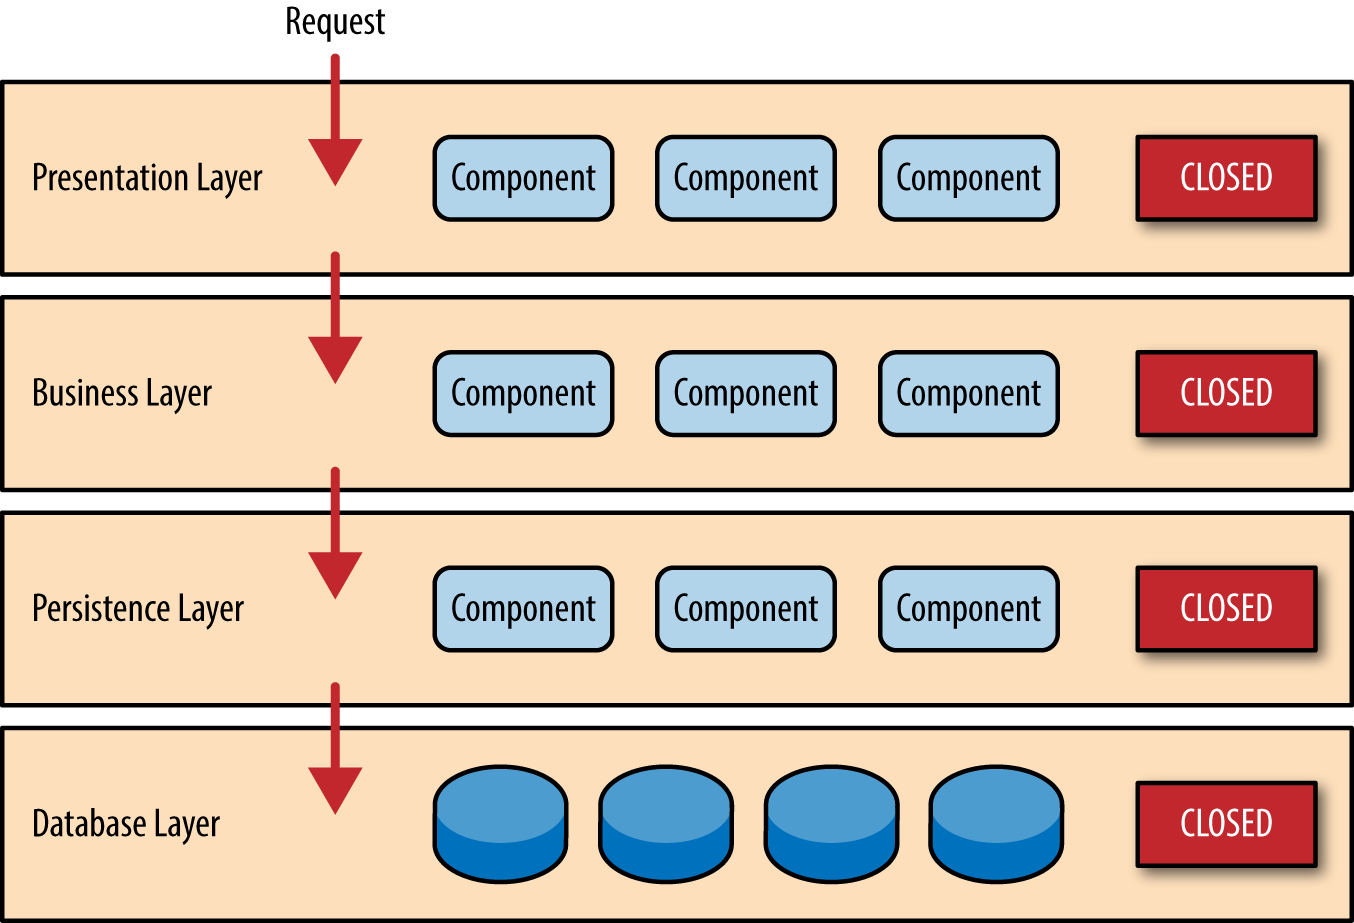
\includegraphics[width=\textwidth]{immagini/layered_archiecture.png}
    \caption{Architettura monolitica a strati}
    \label{fig:layered_architecture}
\end{figure}

\subsection{Strato di persistenza}
Nel nostro caso al posto del Database, alla base, c'è il server che espone la rete neurale per le predizioni. Di conseguenza lo strato di persistenza è l'insieme di quelle classi addette a comporre la richiesta HTTP da inviare all'end-point, le quali sono collocate nel package prediction. In particolare all'interno di questo troviamo la classe NeuralNetworkClient che contiene tra i suoi campi dati un oggetto con il tipo HttpClient, offerta dalla libreria \verb|java.net|. Grazie a questo è possibile esporre nell'interfaccia pubblica della classe il metodo \verb|predict|, il quale prende come parametro una lista contenente i valori dello spettro luminoso (già interpolati in modo che siano uniformi con i valori con cui la rete è stata allenata) e ritorna un valore interno $k \in \{0 .. 6 \}$ che indica la classe di appartenenza tra quelle elencate nel capitolo \ref{cap:machine-learning}. Questo metodo ha inoltre il compito di gestire eventuali eccezioni lanciate durante la chiamata al server, ritornando un valore negativo.\\
È possibile vedere il diagramma delle classi per questo layer nella figura \ref{fig:class_diagram_persistence}.

\begin{figure}
    \centering
    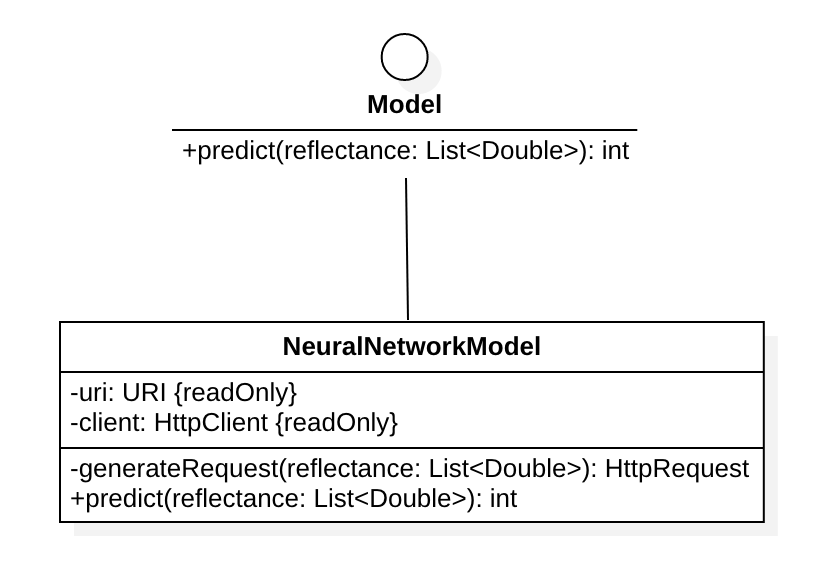
\includegraphics[width=0.8\textwidth]{immagini/model_classes.png}
    \caption{Diagramma delle classi per lo strato di persistenza}
    \label{fig:class_diagram_persistence}
\end{figure}

\subsection{Strato di business}
Salendo, a questo livello, troviamo l'insieme delle classi atte al calcolo del percorso che il drone dovrà eseguire. Si riporta nell'algoritmo \ref{alg:calculate_track} lo pseudocodice per il calcolo del percorso. L'input sono due array paralleli $x$ e $y$ di grandezza $n$ (con $n$ il numero di punti da attraversare) contenenti le coordinate. Indossando un altro paio di occhiali, possiamo notare come questo problema è riconducibile ad un \textit{grafo completo} $K_n$, in cui ogni nodo è connesso da un arco a tutti gli altri. Ognuno di questi archi ha un costo di percorrenza che dipende direttamente dalla distanza tra i due punti, espressi in coordinate. Ci troviamo di fronte al problema del commesso viaggiatore.\\
È possibile vedere il diagramma delle classi per questo layer nella figura \ref{fig:class_diagram_business}.

\begin{figure}
    \centering
    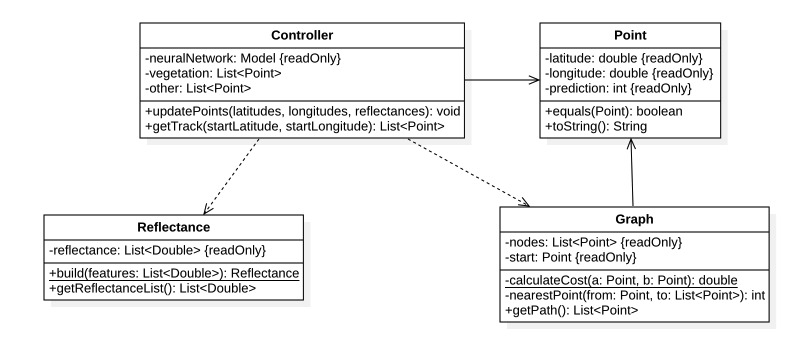
\includegraphics[width=\textwidth]{immagini/business_classes.png}
    \caption{Diagramma delle classi per lo strato di business}
    \label{fig:class_diagram_business}
\end{figure}

\subsubsection{Problema del commesso viaggiatore}
Il nome nasce da una tipica rappresentazione del problema: dato un insieme di città da visitare una ed una sola volta e note le distanze tra queste, trovare il tragitto di minima percorrenza che un commesso viaggiatore deve eseguire per effettuare tutte le consegne e ritornare al punto di partenza. È stato dimostrato che questo problema è \textit{NP-hard}, in quanto non esiste un algoritmo che lo risolva in tempo polinomiale. L'unico metodo di risoluzione efficace è l'enumerazione totale dei possibili percorsi, che ricade nella classe di complessità computazionale $\theta(n!)$.

\subsubsection{Algoritmo euristico di risoluzione}
Per affrontare il problema si è deciso di realizzare un algoritmo euristico, ovvero la cui soluzione prodotta è probabilmente buona ma non ottima.
Come si può notare, il costo computazionale della procedura \verb|nearest_point| è lineare, dunque il costo totale della procedura rientra nella classe di algoritmi $\theta(n^2)$ con consumo di memoria costante. Considerando che nell'applicazione reale il valore di $n$ non raggiungerà mai valori elevati, il risultato è accettabile. Inoltre è possibile ottimizzare questo algoritmo durante l'implementazione rimuovendo i punti già inclusi nel cammino dagli array $x$ e $y$ al posto di porre le coordinate a infinito.

\begin{algorithm}
    \caption{Algoritmo per il calcolo del percorso}
    \label{alg:calculate_track}
    \begin{algorithmic}
        \Require array $x[1 \dotso n]$ e $y[1 \dotso n]$ senza valori duplicati
        \Require $x\_start \notin x$ e $y\_start \notin y$
        \Ensure $x\_path[1 \dotso n+1]$ e $y\_path[1 \dotso n+1]$
        \State Inizializza array $x\_path[1 \dotso n+1]$, $y\_path[1 \dotso n+1]$
        \State $x\_prev = x\_start$
        \State $y\_prev = y\_start$
        \For{$i=1$ to $n$}
            \State $next = \verb|nearest_point|(x\_prev,\  y\_prev,\  x,\  y)$
            \Comment Algoritmo \ref{alg:nearest_point}
            \State $x\_path[i] = x[next]$
            \State $y\_path[i] = y[next]$
            \State $x[next] = \infty$
            \State $y[next] = \infty$
            \State $x\_prev = x[i]$
            \State $y\_prev = y[i]$
        \EndFor
        \State $x\_path[n+1] = x\_start$ \Comment Punto di arrivo
        \State $y\_path[n+1] = y\_start$
        \State \Return $(x\_path , y\_path)$
    \end{algorithmic}
\end{algorithm}

\begin{algorithm}
    \caption{Procedura nearest point}
    \label{alg:nearest_point}
    \begin{algorithmic}
        \Require $x\_from$, $y\_from$ il punto di partenza
        \Require $x\_to[1 \dotso n]$, $y\_to[1 \dotso n]$ array con le $n$ destinazioni possibili differenti
        \Ensure $minIndex$ l'indice della posizione più vicina
        \State $minIndex = -1$
        \State $minDistance = \infty$
        \For{$i=1$ to $n$}
            \State $distance = \sqrt{(x\_from - x\_to[i])^2 + (y\_from - y\_to[i])^2}$
            \If{$distance < minDistance$}
                \State $minDistance = distance$
                \State $minIndex = i$
            \EndIf
        \EndFor
        \State \Return $minIndex$
    \end{algorithmic}
\end{algorithm}

\subsection{Strato di presentazione}
Questo livello ha il compito di esporre tutto il monolite all'esterno.
Va premesso che il drone che andrà ad interfacciarsi con questo software avrà una scheda Arduino, dunque in grado di effettuare chiamate HTTP ad un end-point indicato.
Nel nostro specifico caso si tratta di esporne due:
\begin{itemize}
    \item \verb|/track|: questo risponde a chiamate HTTP di tipo GET, viene invocato dal drone quando ha bisogno di conoscere il tracciato che deve percorrere;
    \item \verb|/data|: questo risponde a chiamate HTTP di tipo POST, viene invocato dal drone quando ha fatto delle rilevazioni con lo spettrometro e le invia al software in modo che il percorso di aggiorni. La risposta può essere un successo o un fallimento.
\end{itemize}
È possibile vedere il diagramma delle classi per questo layer nella figura \ref{fig:class_diagram_presentation}.

\begin{figure}
    \centering
    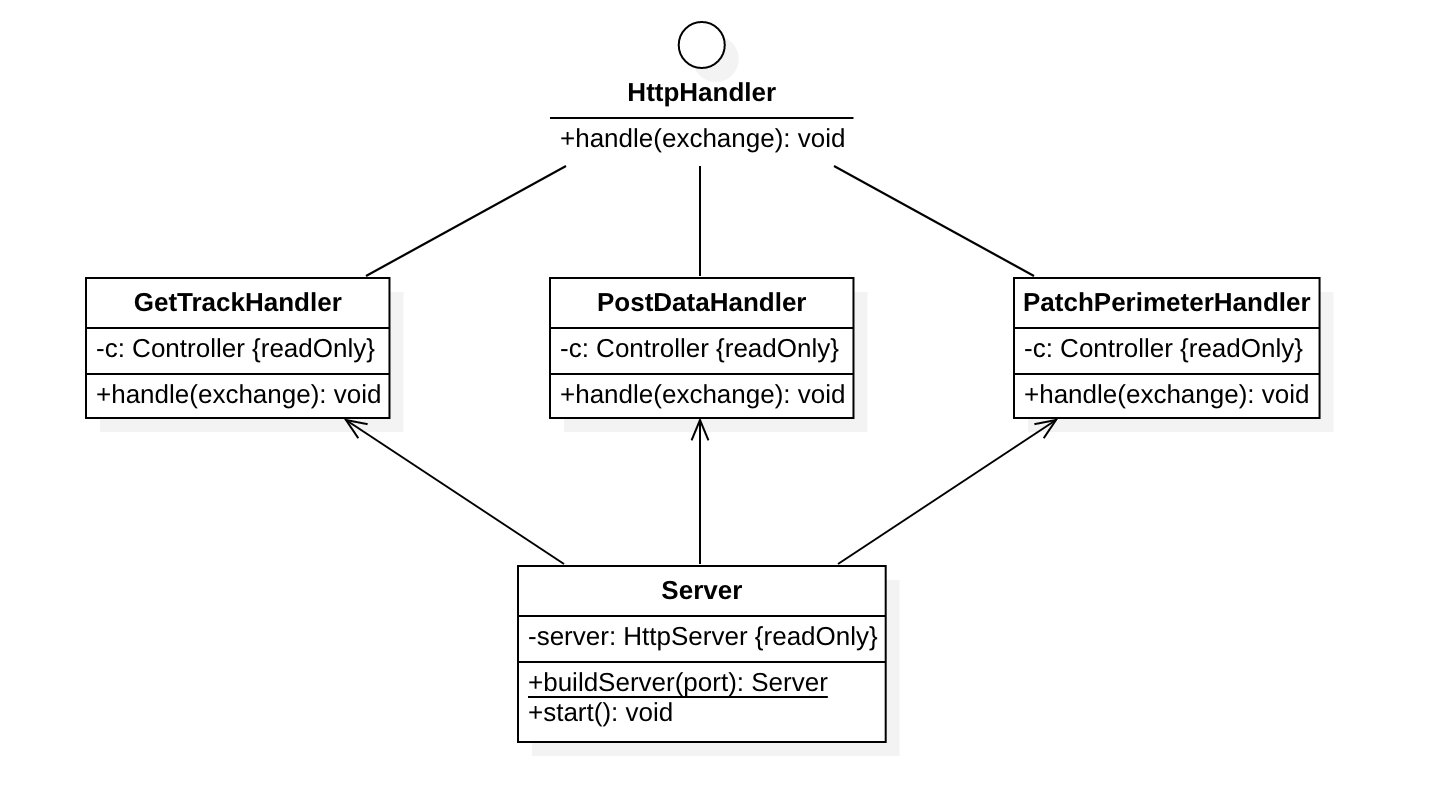
\includegraphics[width=0.8\textwidth]{immagini/presentation_classes.png}
    \caption{Diagramma delle classi per lo strato di presentazione}
    \label{fig:class_diagram_presentation}
\end{figure}